\documentclass[a4paper]{article}

\usepackage[utf8]{inputenc}
\usepackage[T1]{fontenc}
\usepackage{textcomp}
\usepackage[a4paper, total={6in, 8in}]{geometry}
\usepackage[spanish]{babel}
\usepackage{amsmath, amssymb, amsthm, amsfonts, mathabx}
\usepackage{mathtools}
\usepackage{enumitem}
\usepackage{subcaption}
\usepackage{graphicx}
\usepackage{hyperref}
\hypersetup{
  colorlinks=true,
  linkcolor=cyan,
  filecolor=magenta,      
  urlcolor=cyan,
}
\usepackage{cleveref}

\usepackage[
backend=biber,
style=ieee,
sorting=ynt
]{biblatex}
\addbibresource{ref.bib}

\usepackage{xcolor}
\definecolor{codegreen}{rgb}{0,0.6,0}
\definecolor{codegray}{rgb}{0.5,0.5,0.5}
\definecolor{codepurple}{rgb}{0.58,0,0.82}
\definecolor{backcolour}{rgb}{0.96,0.96,0.96}

\usepackage{listings}
\lstdefinestyle{listings_style}{
    backgroundcolor=\color{backcolour},   
    commentstyle=\color{codegreen},
    keywordstyle=\color{magenta},
    numberstyle=\tiny\color{codegray},
    stringstyle=\color{codepurple},
    basicstyle=\ttfamily\footnotesize,
    breakatwhitespace=false,         
    breaklines=true,                 
    captionpos=b,                    
    keepspaces=true,                 
    % numbers=left,                    
    % numbersep=5pt,                  
    showspaces=false,                
    showstringspaces=false,
    showtabs=false,                  
    tabsize=2
}
\lstset{style=listings_style}

\def\eps{\varepsilon}

\newcommand{\dotp}[2]{\left\langle#1,#2\right\rangle}

\newcounter{objects}[section]
\renewcommand{\theobjects}{\thesection.\arabic{objects}}
\newtheorem{theorem}[objects]{Teorema}
\newtheorem{proposition}[objects]{Proposición}
\newtheorem{definition}[objects]{Definición}
\newtheorem{example}[objects]{Ejemplo}
\newtheorem{corollary}[objects]{Corolario}
\newtheorem{lemma}[objects]{Lema}
\newtheorem{remark}[objects]{Observación}

\setlength{\parskip}{1em}

\title{Hito 2 - Análisis de Redes Sociales y Computación Evolutiva y Bioinspirada}
\author{Pablo Miralles González}
\date{\today}

\begin{document}
  \maketitle

  \section{Introducción}

En esta práctica tratamos el problema de detección de comunidades en un grafo
de artículos de Amazon, donde contamos con el \emph{ground truth} dado por las
categorías de los mismos para evaluar los resultados obtenidos. Esta memoria
se divide en tres partes principales. En la sección \ref{sec:ej1} se responden
a las cuestiones propuestas en el primer ejercicio. En la sección \ref{sec:ej2}
se detalla la metodología seguida para seleccionar la configuración del algoritmo
\emph{NSGA-II}, junto con la configuración final. Por último, en la sección
\ref{sec:ej3} se analizan los resultados del ejercicio anterior, y se responden
a las cuestiones del tercer ejercicio.

El código fuente de la práctica se encuentra en el repositorio de GitHub
\href{https://github.com/pablomiralles22/maadm-sna-ceb-assignment}{pablomiralles22/maadm-sna-ceb-assignment}. En el fichero \lstinline{README.md} se explica la estructura del
código, y cómo ejecutarlo para replicar los pasos seguidos en esta práctica.


  \section{Ejercicio 1}\label{sec:ej1}

Tras aplicar el algoritmo de Leiden a la red de artículos de Amazon, se obtiene
una partición de 18 comunidades, con una modularidad de $0.8832$. Sin embargo,
al comparar mediante la información mutua normalizada con el \emph{ground truth},
encontramos un resultado de $0.54$, que es bastante bajo.

En la figura \ref{fig:1-circular-comp} podemos comparar los gráficos circulares
del \emph{ground truth} y de la salida del algoritmo de Leiden, usando el color
para representar la intersección entre comunidades de las dos soluciones. En la
figura \ref{fig:1-bipartite} podemos ver una comparación mediante un grafo
bipartito, donde los nodos de la izquierda representan las comunidades
\emph{ground truth}, los de la derecha las comunidades generadas por el
algoritmo de Leiden. En esta figura, las aristas representan la intersección
entre comunidades, y los colores de los nodos de la derecha también.

Vemos que la comunidad real más grande se ha dividido en muchas. También que
otras tres comunidades pequeñas quedan divididas (en 2, 2 y 3 comunidades).
Además, en general las comunidades generadas por Leiden se corresponden a una
sola comunidad original. Esto se da en 13 de 18 comunidades.

\begin{figure}[!htb]
  \centering
  \begin{subfigure}{.4\textwidth}
    \centering
    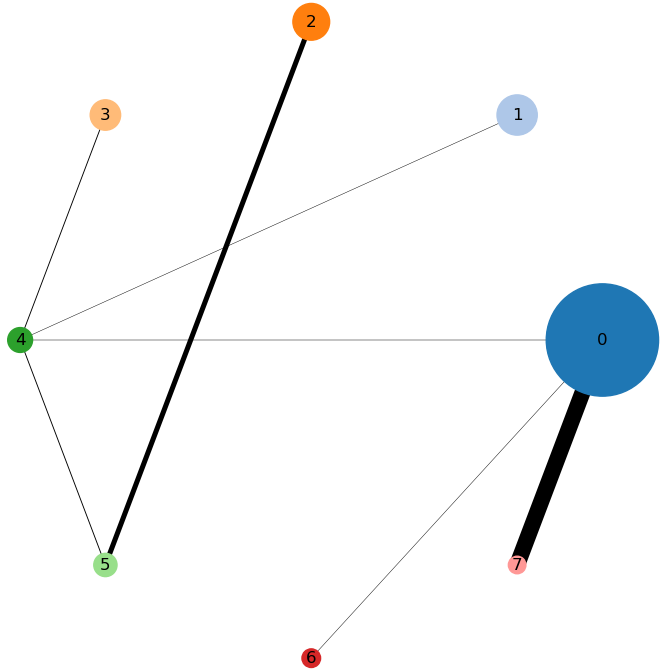
\includegraphics[width=.9\linewidth]{img/1_circular_comp_1}
    \caption{Gráfico circular de las comunidades \emph{ground truth}. }
    \label{fig:1-circular-comp-1}
  \end{subfigure}%
  \hfill
  \begin{subfigure}{.4\textwidth}
    \centering
    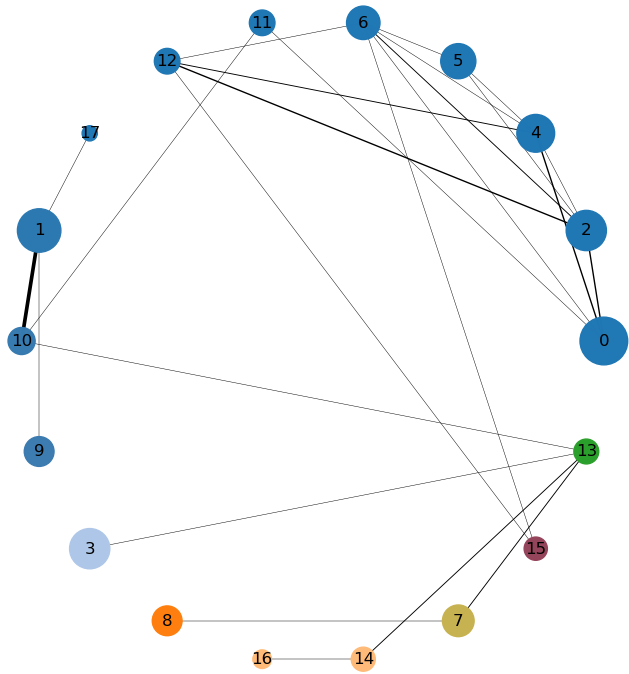
\includegraphics[width=.9\linewidth]{img/1_circular_comp_2}
    \caption{Gráfico circular de las comunidades generadas por el algoritmo de Leiden. }
    \label{fig:1-circular-comp-2}
  \end{subfigure}
  \caption{Comparación de gráficos circulares entre el \emph{ground truth} y el
    algoritmo de Leiden. Los colores de las comunidades en el gráfico de la
    derecha son una media de los del gráfico de la izquierda, en función del
    tamaño de la intersección con la comunidad correspondiente.}
  \label{fig:1-circular-comp}
\end{figure}

\begin{figure}[!htb]
  \centering
  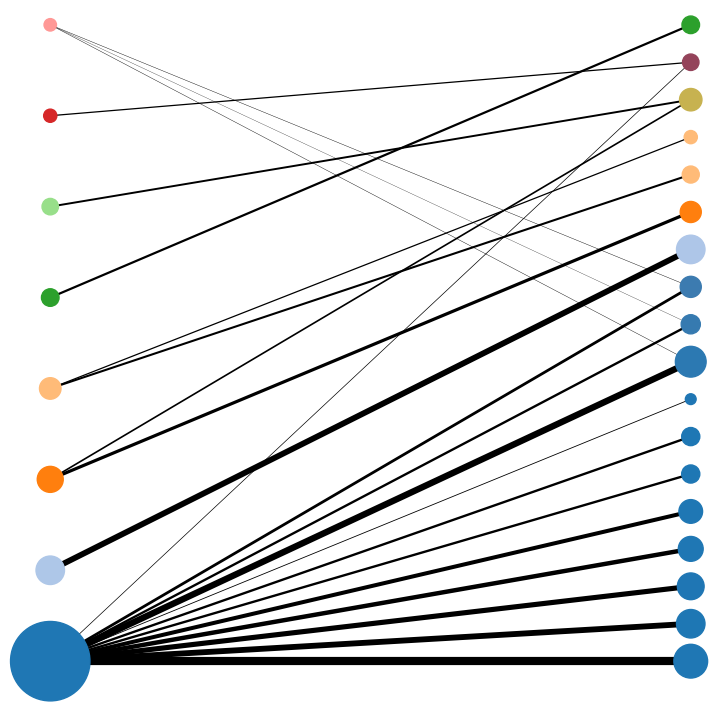
\includegraphics[width=.7\linewidth]{img/1_bipartite_comp}
  \caption{Comparación de comunidades mediante un grafo bipartito. A la
    izquierda vemos las comunidades \emph{ground truth}, y a la derecha las
    generadas por el algoritmo de Leiden.  Los colores de las comunidades en el
    gráfico de la derecha son una media de los del gráfico de la izquierda, en
    función del tamaño de la intersección con la comunidad correspondiente. Los
    tamaños de las aristas son tan gruesos como el número de nodos en común de las
    comunidades que conectan.}
  \label{fig:1-bipartite}
\end{figure}



Todo parece indicar un problema de resolución, como hemos visto en clase.
Recordemos que la fórmula de la modularidad se puede escribir como:
$$
\sum_{i=1}^C e_{ii} - a_i^2,
$$
donde
\begin{itemize}
  \item $e_{ij}$ es la fracción de aristas con un vértice en la comunidad $i$ y
    el otro en la $j$.
  \item $a_i$ es la fracción de aristas con algún vértice en la comunidad $i$.
\end{itemize}

Si nos fijamos, el primer término es $\sum_i e_{ii} = 1 - \sum_{i\neq j}
e_{ij}$, es decir, que para maximizar el primer término buscamos minimizar la
fracción de aristas entre comunidades. Es claro que para ello nos conviene
tener pocas y grandes comunidades. En el caso extremo, si solo hubiese una
comunidad obtendríamos el valor perfecto $1$. Respecto al segundo término, se
puede descomponer como:
$$
\sum_{i=1}^C a_i^2 =
\frac{1}{(2m)^2} \sum_{i=1}^C \left( \sum_{n \in c_i} \delta(n)^2 + \sum_{n_1, n_2 \in c_i, n_1 \neq n_2} \delta(n_1) \delta(n_2) \right) 
.$$
La suma de los cuadrados es imposible de evitar, y el otro término depende de
los grados de nodos en la misma comunidad. Si los grados son bajos, se
considera que es poco probable que los nodos se crucen entre sí, y por lo tanto
una conexión entre ellos es significativa. Por lo tanto, se buscan comunidades
con pocos nodos y cuyos grados sean pequeños. En el caso extremo, si cada nodo
formase una comunidad, este término se minimizaría. Es fácil ver entonces que
esta métrica busca un mayor número de comunidades.

Este \emph{trade-off} se suele modular con un parámetro positivo $\gamma > 0$,
de la siguiente forma:
$$
\sum_{i=1}^C e_{ii} - \gamma a_i^2
.$$
Cuando $\gamma$ es grande, el algoritmo tiende a dividir comunidades grandes, y
en caso contrario a juntar comunidades pequeñas.

Con esta consideración, podemos probar a ejecutar el algoritmo de Leiden con
con diferentes valores de $\gamma$. Como la implementación no lo permite,
recurro en esta parte al algoritmo menos avanzado de Louvain. En la figura
\ref{fig:1-resolution-vs-nmi} podemos ver la información mutua normalizada con
el \emph{ground truth} en función del parámetro $\gamma$. Vemos que el valor
máximo se alcanza en $\gamma = 0.06$, con un valor ligeramente
superior a $0.7$. En la figura \ref{fig:1-best_res_bipartite} podemos ver una
comparación de las comunidades obtenidas con este valor de $\gamma$. En este caso,
vemos que la comunidad grande se divide en solo tres comunidades, lo cual es una
gran mejora, pero sigue sin llegar a juntarse en una. Además, las comunidades
reales más pequeñas las junta con esas tres que corresponden a la más grande.
Finalmente, vemos que dos parejas de comunidades reales medianas quedan juntas.

Observamos que hemos pasado de un extremo a otro salvo con la comunidad más
grande. Con una resolución alta, el algoritmo separaba las comunidades
demasiado, y con una resolución baja, tiende a juntarlas demasiado. Por lo
tanto, no parece que podamos recuperar la estructura original mediante estos
algoritmos, ni siquiera tratando de seleccionar la resolución correcta. Esto
ocurre porque distintas partes de la estructura de red requieren distintas
resoluciones, pero esto no se puede saber a priori sin el \emph{ground truth}.
Este problema con algunos métodos multi-resolución ya fue evaluado por
\citeauthor{lancichinetti2011Limitsmodularity}
\cite{lancichinetti2011Limitsmodularity}: \emph{"We show that multiresolution
modularity suffers from two opposite coexisting problems: the tendency to merge
small subgraphs, which dominates when the resolution is low; the tendency to
split large subgraphs, which dominates when the resolution is high"}.

\begin{figure}[!htb]
  \centering
  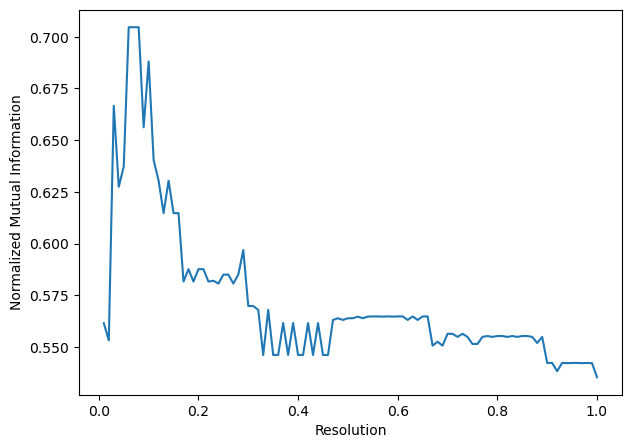
\includegraphics[width=.7\linewidth]{img/1_resolution_vs_nmi}
  \caption{Comparación de la información mutua normalizada con el \emph{ground}
    \emph{truth} en función del parámetro $\gamma$ del algoritmo de Louvain.}
  \label{fig:1-resolution-vs-nmi}
\end{figure}

\begin{figure}[!htb]
  \centering
  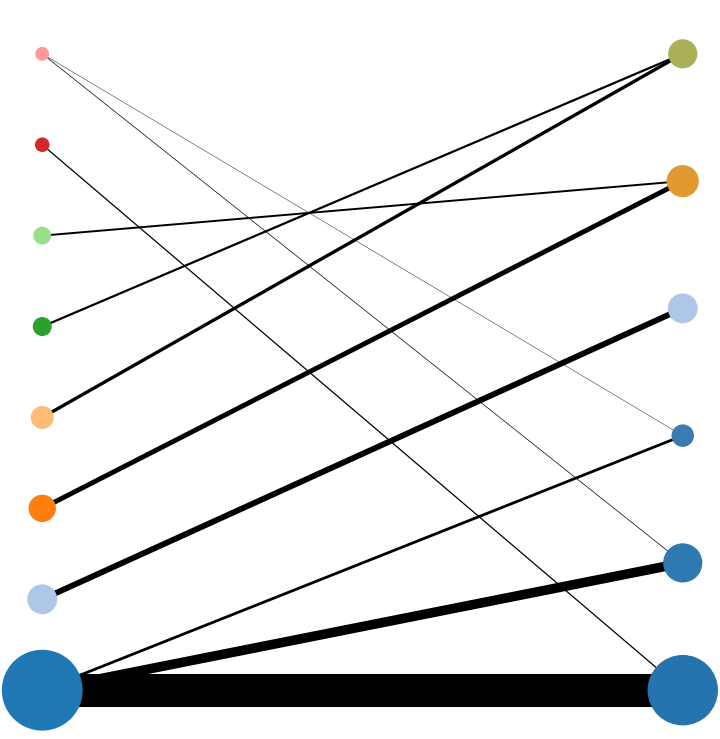
\includegraphics[width=.7\linewidth]{img/1_best_res_bipartite_comp}
  \caption{Comparación de comunidades mediante un grafo bipartito. A la
    izquierda vemos las comunidades \emph{ground truth}, y a la derecha las
    generadas por el algoritmo de Lovain con \(\gamma=0.06\).  Los colores de
    las comunidades en el gráfico de la derecha son una media de los del
    gráfico de la izquierda, en función del tamaño de la intersección con la
    comunidad correspondiente. Los tamaños de las aristas son tan gruesos como
    el número de nodos en común de las comunidades que conectan.}
  \label{fig:1-best_res_bipartite}
\end{figure}



  \section{Ejercicio 2}\label{sec:ej2}

Pasamos entonces a la resolución con algoritmos genéticos muti-objetivo. Para
ello, implemento el algortimo NSGA-II, según se describe en el artículo de
\citeauthor{deb2002fastelitist} \cite{deb2002fastelitist}. Respecto al diseño,
se toman las siguientes decisiones:

\begin{description}
  \item[Representación.] Se usa la representación \emph{locus adyacency}, como
    obligaba la práctica.
  \item[Funciones objetivo.] Basado en los resultados de
    \citeauthor{shi2014Comparisonselection} \cite{shi2014Comparisonselection},
    buscamos dos funciones objetivo que estén correlacionadas negativamente,
    de manera que sean objetivos contrapuestos: mejorar uno empeora el otro.
    El problema se convierte entonces en encontrar un compromiso entre ambos.
    Uso las siguientes funciones objetivo:
    \begin{itemize}
      \item \textbf{Densidad interna media de las comunidades}. Busca que los nodos de
        la misma comunidad estén muy conectados entre sí. Si una comunidad tiene
        \(n\) nodos y \(m\) aristas, la densidad interna es \(2m/(n(n-1))\), ya que
        el número máximo de aristas posible es \(n(n-1)/2\). Por lo tanto, la métrica
        se calcula como:
        $$
        \frac{1}{|C|} \sum_{S \in C} \frac{m_s}{(n_s \cdot (n_s-1)) / 2}
        .$$

      \item \textbf{\emph{Average out degree fraction.}} Dada una comunidad \(S\),
        definimos \(I_S = \{ (u,v): u,v\in S \}\) como el conjunto de aristas internas
        a \(S\), y \(T_S = \{ (u,v): u\in S \text{ o } v \in S\}\) como el conjunto
        de aristas que tienen al menos un extremo en \(S\). La fracción de aristas
        que apuntan al exterior de \(S\) es entonces \(1 - |I_S| / |T_S|\). La métrica
        se calcula entonces como:
        $$
        \frac{1}{|C|} \sum_{S \in C} \left(1 - \frac {|I_S|} {|T_S|} \right)
        ,$$
        donde en este caso buscamos minimizar.
    \end{itemize}

    Estas dos métricas es claro que se contraponen. Cuantos más nodos añadimos a una
    comunidad, más difícil es que todos estén bien conectados entre si, y por lo tanto
    la densidad interna disminuye. Por otro lado, cuantos más nodos tenga una
    comunidad, menos potenciales aristas hacia fuera de dicha comunidad tendrá. En el
    caso extremo, una sola comunidad nos da \(0\) de \emph{average out degree fraction},
    mientras que si tenemos \(n\) comunidades, cada una con un solo nodo, cada comunidad
    tendría densidad interna máxima.

    En el artículo citado estas dos métricas aparecen correlacionadas positivamente,
    porque una se minimiza y la otra se maximiza. En este caso, mi algoritmo solo maximiza,
    de forma que trabajaré con \(1 - AVG\_ODF\) en lugar de con \(AVG\_ODF\).

  \item[Operadores de selección.] Usaré selección por torneo, minimizando el rango (número
    del frente de Pareto al ordenar por dominancia e ir extrayendo los frentes) y maximizando
    en segunda instancia la distancia de Crowding, como se indica en \cite{deb2002fastelitist}.

  \item[Operadores de cruce.] Usaré un cruce por máscara aleatoria, donde los elementos
    a \lstinline{True} serán intercambiados y los otros no. Usar operados de cruce que
    atiendan a la posición de los genes creo que no tiene sentido, ya que en un grafo el
    orden de los nodos no importa, y las operaciones deberían ser invariantes a la
    permutación de los nodos.

  \item[Operadores de mutación.] Usaré una combinación de tres mutaciones distintas. Cada
    vez que se muta a un individuo, se elige una al azar. Son las siguientes:
    \begin{itemize}
      \item \lstinline{random(ratio)}. Cada gen se muta con probabilidad
        \lstinline{ratio} por otro vecino aleatorio del nodo.

      \item \lstinline{join(ratio)}. Consideramos ahora solo los nodos cuyo gen
        es él mismo o apunta a otro gen que le apunta de vuelta. En estos casos,
        el nodo está en una comunidad con uno o dos nodos. Para cada uno
        de estos, se muta con probabilidad \lstinline{ratio} por un vecino
        aleatorio del nodo.

      \item \lstinline{separate(ratio)}. Para cada nodo, con probabilidad
        \lstinline{ratio} se muta por él mismo, rompiendo entonces un enlace
        y posiblemente separando la comunidad en dos.
    \end{itemize}

    Al introducir estas tres mutaciones con parámetros, permite dar más o menos
    peso a cada una, e integrarlas en la medida que mejor resultados obtenga.
    Al poder optimizar estos hiperparámetros, el algoritmo podrá adaptar el
    nivel de exploración en zonas de comunidades grandes o pequeñas. Estos
    hiperparámetros se seleccionarán evaluando los frentes de Pareto con
    distintas métricas, mediante la librería de Python \lstinline{optuna}.
\end{description}

Los parámetros optimizados con \lstinline{optuna} se muestran en la
Tabla~\ref{tab:ej2-params}, junto con las posibilidades consideradas y los
valores seleccionados finalmente. Para su selección se consideran las métricas
de \emph{hipervolumen} y \emph{dispersión de Zitzler} vistas en clase. El
algoritmo devuelve un nuevo frente de Pareto con estas métricas, y selecciono
una solución intermedia de compromiso arbitraria. Se realizan en total \(120\)
pruebas de hiperparámetros, con \(5000\) llamadas a la función de
\emph{fitness} y un solo experimento por cada una. Serían necesarios varios
experimentos para cada combinación de hiperparámetros, obteniendo una media de
las métricas, pero esto es demasiado costoso computacionalmente.

\begin{table}[!htbp]
\centering
\begin{tabular}{|r||cccc|}
\hline
Parámetro                       & Tipo    & Rango         & Paso & Valor seleccionado \\\hline
Tamaño de población             & Entero  & $[25, 150]$ & $25$   & $50$                 \\
Probabilidad de cruce           & Decimal & $[0.5, 1]$  & $0.05$ & $0.55$               \\
Probabilidad de mutación        & Decimal & $[0, 0.5]$  & $0.05$ & $0.1$                \\
Ratio de mutación aleatoria     & Decimal & $[0, 0.2]$  & -    & $0.0047$             \\
Ratio de mutación de unión      & Decimal & $[0, 1]$    & -    & $0.86$               \\
Ratio de mutación de separación & Decimal & $[0, 0.2]$  & -    & $0.012$              \\
T (candidatos por torneo)       & Entero  & $[2, 16]$   & -    & $4$                  \\\hline
\end{tabular}
\caption{Hiperparámetros optimizados y seleccionados para el algoritmo NSGA-II.}
\label{tab:ej2-params}
\end{table}



  \section{Ejercicio 3}\label{sec:ej3}

Evaluamos en esta sección el frente de Pareto de soluciones obtenido.
Consideramos primero la forma de las soluciones obtenidas, a grandes rasgos. En
la figura \ref{fig:3-pareto-num-coms-1} vemos el frente de Pareto obtenido,
junto con el número de comunidades en cada solución. Como esperábamos, cuanto
más se prioriza la densidad interna, en más comunidades se dividen los nodos, y
al revés con el \emph{average out-degree fraction}.

\begin{figure}[!htb]
  \centering
  \begin{subfigure}{.48\textwidth}
    \centering
    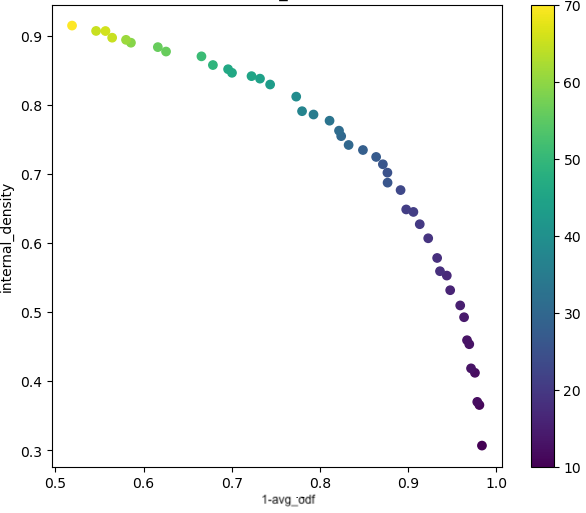
\includegraphics[width=\linewidth]{img/3_num_communities_pareto_1}
    \caption{Gráfico de los valores de \emph{fitness} de las soluciones del
    frente de Pareto obtenido. El eje $x$ representa el \(1-AVG\_ODF\), y el
    eje \(y\) la densidad interna media. El color representa el número de
    comunidades producidas.}
    \label{fig:3-pareto-num-coms-1}
  \end{subfigure}%
  \hfill
  \begin{subfigure}{.48\textwidth}
    \centering
    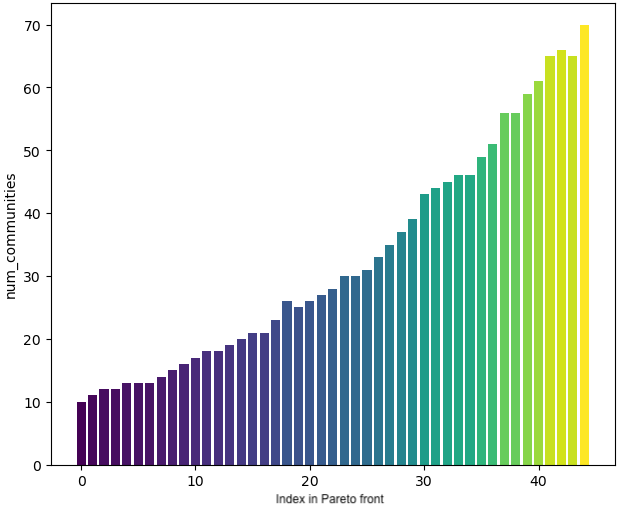
\includegraphics[width=\linewidth]{img/3_num_communities_pareto_2}
    \caption{Gráfico de barras del número de comunidades producidas. Las
      soluciones del frente de Pareto están ordenadas de menor \emph{average
      out-degree fraction} (izquierda) a mayor densidad interna (derecha). El
      eje \(y\) y el color representan la el valor de la información mutua
      respecto al \emph{ground truth}.}
  \label{fig:3-pareto-num-coms-2}
  \end{subfigure}
  \caption{Comparación del número de comunidades de las soluciones del frente
  de Pareto.}
  \label{fig:3-pareto-num-coms}
\end{figure}

Respecto a la información mutua con el \emph{ground truth}, vemos en la figura
\ref{fig:3-pareto-nmi-1} la comparación de dicha métrica entre las soluciones
del frente de Pareto. Es fácil ver que en general funciona mejor priorizar
bastante el \emph{average out-degree fraction}. Cogiendo la mejor solución
respecto a la información mutua, vemos en la figuras
\ref{fig:3-circle-comp,fig:3-bipartite} la comparación de las comunidades
obtenidas con las del \emph{ground truth}. Observamos una solución ligeramente
peor que la obtenida \emph{tuneando} el parámetro de resolución en el algoritmo
de Louvain, tanto por el valor de la información mutua (\(0.6788 \leq 0.7\))
como gráficamente.

\begin{figure}[!htb]
  \centering
  \begin{subfigure}{.48\textwidth}
    \centering
    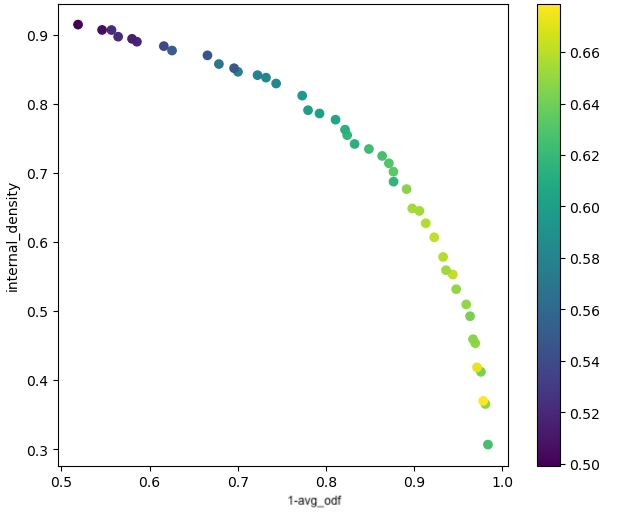
\includegraphics[width=\linewidth]{img/3_nmi_pareto_1}
    \caption{Gráfico de los valores de \emph{fitness} de las soluciones del
    frente de Pareto obtenido. El eje $x$ representa el \(1-AVG\_ODF\), y el
    eje \(y\) la densidad interna media. El color representa el valor de la
    información mutua respecto al \emph{ground truth}.}
    \label{fig:3-pareto-nmi-1}
  \end{subfigure}%
  \hfill
  \begin{subfigure}{.48\textwidth}
    \centering
    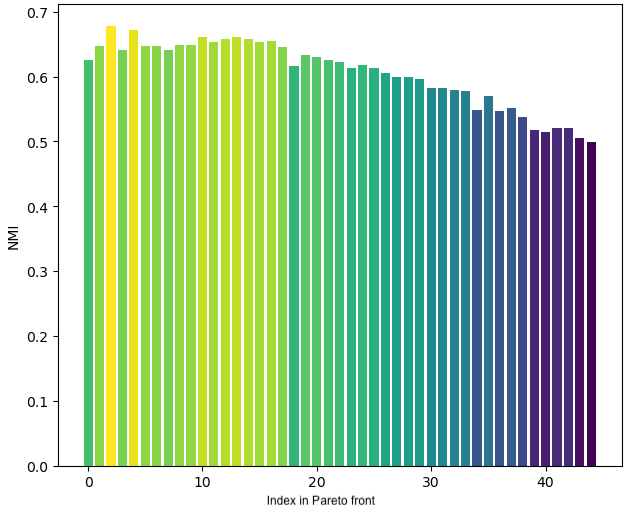
\includegraphics[width=\linewidth]{img/3_nmi_pareto_2}
    \caption{Gráfico de barras de la información mutua respecto al \emph{ground
      truth}. Las soluciones del frente de Pareto están ordenadas de menor
      \emph{average out-degree fraction} (izquierda) a mayor densidad interna
      (derecha). El eje \(y\) y el color representan la el valor de la
      información mutua respecto al \emph{ground truth}.}
  \label{fig:3-pareto-nmi-2}
  \end{subfigure}
  \caption{Comparación de la información mutua respecto al \emph{ground truth}
  de las soluciones del frente de Pareto.}
  \label{fig:3-pareto-nmi}
\end{figure}

\begin{figure}[!htb]
  \centering
  \begin{subfigure}{.4\textwidth}
    \centering
    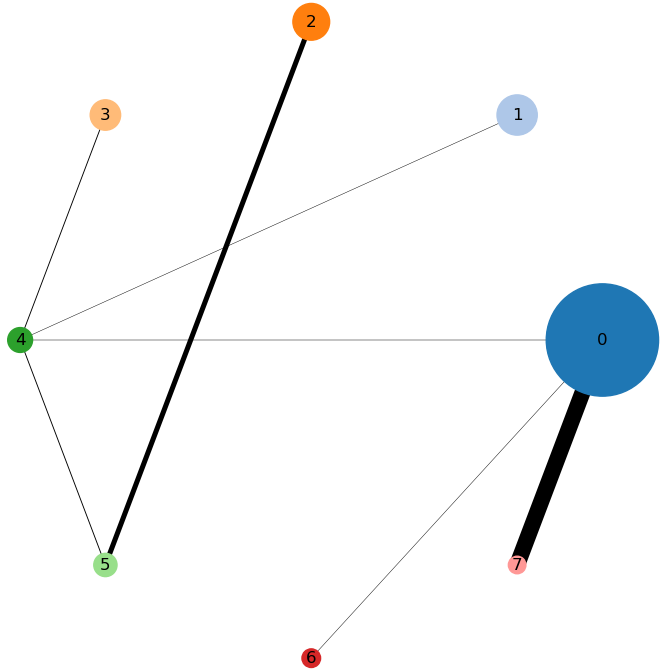
\includegraphics[width=.9\linewidth]{img/1_circular_comp_1}
    \caption{Gráfico circular de las comunidades \emph{ground truth}. }
    \label{fig:3-circular-comp-1}
  \end{subfigure}%
  \hfill
  \begin{subfigure}{.4\textwidth}
    \centering
    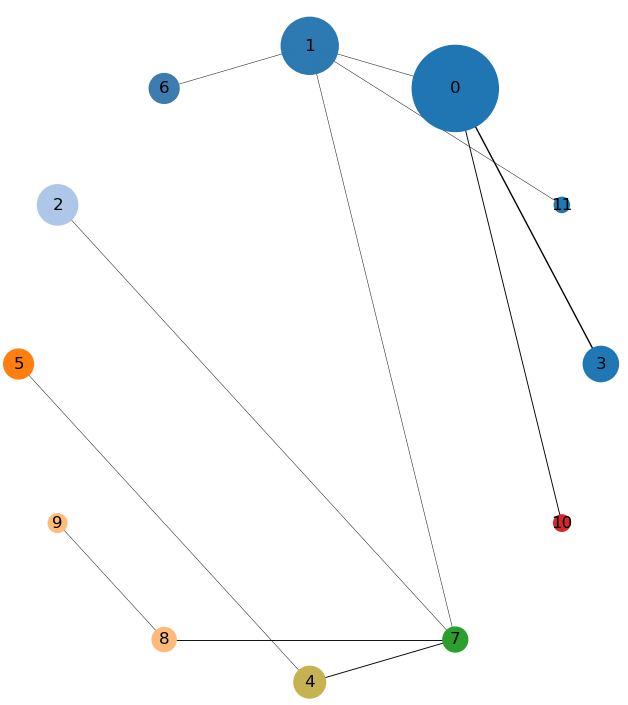
\includegraphics[width=.9\linewidth]{img/3_best_sol_circular_comp_2}
    \caption{Gráfico circular de las comunidades generadas por el algoritmo de Leiden. }
    \label{fig:3-circular-comp-2}
  \end{subfigure}
  \caption{Comparación de comunidades mediante un grafo bipartito. A la
    izquierda vemos las comunidades \emph{ground truth}, y a la derecha la
    mejor solución según la información mutua generada por \emph{NSGA-II}. Los
    colores de las comunidades en el gráfico de la derecha son una media de los
    del gráfico de la izquierda, en función del tamaño de la intersección con la
    comunidad correspondiente.}
  \label{fig:3-circular-comp}
\end{figure}

\begin{figure}[!htb]
  \centering
  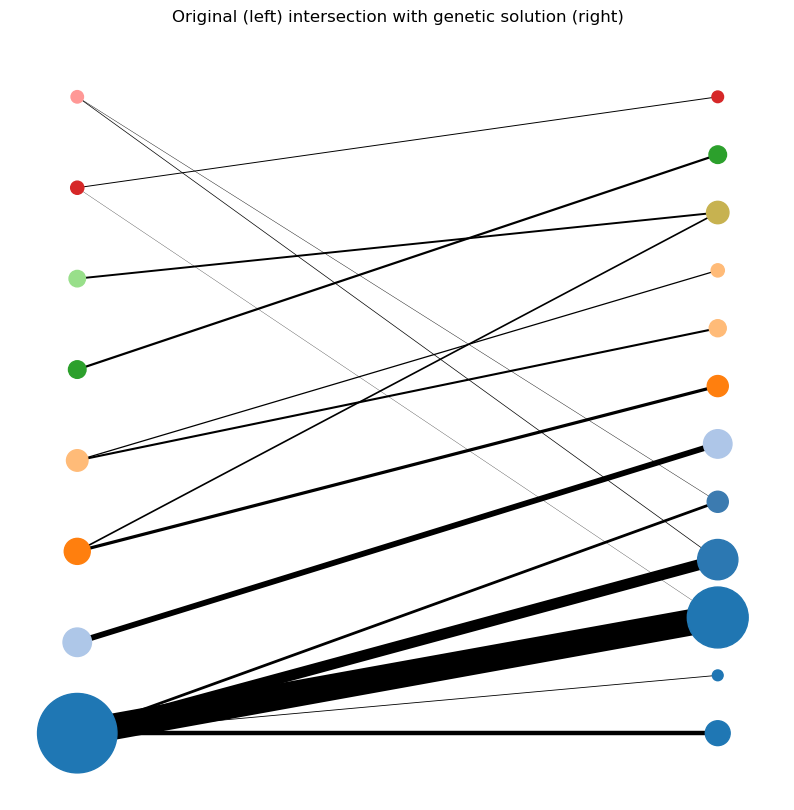
\includegraphics[width=.7\linewidth]{img/3_best_sol_bipartite_comp}
  \caption{Comparación de comunidades mediante un grafo bipartito. A la
    izquierda vemos las comunidades \emph{ground truth}, y a la derecha la
    mejor solución según la información mutua generada por \emph{NSGA-II}. Los
    colores de las comunidades en el gráfico de la derecha son una media de los
    del gráfico de la izquierda, en función del tamaño de la intersección con
    la comunidad correspondiente. Los tamaños de las aristas son tan gruesos
    como el número de nodos en común de las comunidades que conectan.}
  \label{fig:3-bipartite}
\end{figure}

  \section{Conclusiones}
En esta práctica se ha estudiado la detección de comunidades en redes sociales,
en particular en un grafo de artículos de Amazon. En particular:

\begin{itemize}
  \item Se ha resuelto el problema mediante algoritmos voraces, como el
    algoritmo de Leiden y de Louvain para diferentes parámetros de resolución.
  \item Se ha observado el problema de resolución de la métrica de modularidad,
    así como la imposibilidad de resolver el problema independientemente del
    uso de hiperparámetros optimizados cuando las comunidades no están balanceadas
    y requieren resoluciones distintas.
  \item Se ha aplicado un algoritmo genético para la resolución del problema de
    detección de comunidades. En particular, el algoritmo multi-objetivo
    \emph{NSGA-II} con dos métricas contrapuestas seleccionadas. Se han
    estudiado las soluciones del frente de Pareto obtenido, con resultados
    buenos pero no completamente parecidos a las comunidades reales.
  \item De forma trasversal, se han puesto en práctica técnicas de visualización
    de datos apropiadas para grafos y comunidades, intentado una transmisión
    clara de los resultados obtenidos.
\end{itemize}

En general, ha sido una práctica bastante enriquecedora en cuanto a aprendizaje
de técnicas de visualización y de algoritmos y métricas de detección de
omunidades, y de optimización multi-objetivo.





  \clearpage
  \printbibliography[
    heading=bibintoc,
    title={Referencias}
  ]
\end{document}
